\chapter{Results}
\label{ch:chapter5}
\glsresetall

\section{Platform and Software}
\label{sub:platform-software}
I ran the \OpenMC simulation on Sawtooth, a supercomputer at
\Gls{inl}. On Sawtooth, the compute nodes have 2 Intel Xeon 8268 CPUs with 24 cores per
CPU. Hyper-threading is disabled on compute nodes. Each node has 192 GB of RAM.
The login nodes have the same specifications. See Table \ref{tab:sawtooth-params}
for the full specifications of the machine. To avoid any potential licensing
issues with getting \SerpentTWO on Sawtooth, I performed the \SerpentTWO runs
on my office computer, a Dell Precision 3430 Workstation, using 12 OpenMP threads.

\begin{table}[htpb] 
    \centering 
    \caption{Sawtooth job parameters for 100k particle \OpenMC run}
    \label{tab:sawtooth-params}
    \begin{tabular}{|c|c|} 
        \hline
        Quantity & Value\\
        \hline
        Nodes & 92 \\
        \hline
        MPI processes per node & 6 \\
        \hline
        Threads per core & 1 \\
        \hline
        OpenMP threads per MPI process & 8 \\
        \hline
    \end{tabular}
\end{table}
% make this subsection a table

\subsection{Simulation Design and Parameters}
\label{sub:simulation-parameters}

The purpose of these simulations is to test the accuracy of
the implementation of \OpenMC support, so we do not need to do as detailed an
analysis as Ryhlevskii did on finding the equilibrium state. A moderate amount
of timesteps will suffice. I decided to use the same 3 day timesteps as Ryhklevskii
\cite{rykhlevskii_modeling_2019} (as discussed in Section \ref{sub:reprocessing-system-model})
for a year's worth of runtime. Table \ref{tab:saltproc-params} summarizes the simulation
settings used for both the \SerpentTWO and \OpenMC simulations. While I had intended
to use interpolated fission product yields for both the \OpenMC and \SerpentTWO simulations,
I realized very late into the process of writing this manuscript that I had forgotten to set
that option in \OpenMC. This may be one of the reasons some results have larger errors than expected.
 
\begin{table}[htpb] 
    \centering 
    \caption{Neutronics and Depletion parameters for \SaltProc}
    \label{tab:saltproc-params}
    \begin{tabular}{|c|c|} 
        \hline
        Batches & 200 \\
        \hline
        Inactive batches & 80 \\
        \hline
        Particles per batch & 1e6 \\
        \hline
        Power [W] & 2.25e9 \\
        \hline
        Depletion steps & 122 \\
        \hline
        Depletion step length [days] & 3 \\
        \hline
        Depletion equation solver & IPF CRAM 48 \\
        \hline
        Time integration method & Euler's Method \\
        \hline
    \end{tabular}
\end{table}

\subsection{Data}
\label{sub:results-xs-data}

To ensure consistent results between the \OpenMC and \SerpentTWO coupled
simulations, I must make sure both simulations use the exact same set of data.
For a depletion simulation, This extends beyond simply using the same set of
cross section data. Most of the procedure I describe below is a reproduction of
work done by Romano et al (2019) \cite{romano_depletion_2021}, as well as of
data and scripts found at \url{https://github.com/openmc-dev/data/tree/master/depletion}.

In \SerpentTWO, the default energy release per fission value for \ce{^{235}U}
is set to 202.27 MeV. The energy release per fission (the fission Q-value) values for other actinides
are scaled based on the Q-values in the neutron reaction sublibrary data (MT=3 in the
ENDF evaluation).\footnote{see \url{https://serpent.vtt.fi/mediawiki/index.php/Input_syntax_manual\#set_fissh}}
To ensure \OpenMC and \SerpentTWO use the same Q-values for actinides, 
I used the Q-values calculated by Romano et al (2019) for the {\bf endfb71x} library,
available at \url{https://github.com/openmc-dev/data/blob/master/depletion/serpent_fissq.json}.
If the Q-values fer not the same, the power normalization would be different
between the two codes,
resulting in different depletion rates \cite{romano_depletion_2021}.

\SerpentTWO also uses constant valued branching ratios for long-lived metastable
nuclides.\footnote{see \url{https://serpent.vtt.fi/mediawiki/index.php/Default_isomeric_branching_ratios}}
I set the branching ratios in my \OpenMC depletion chain to match the default
values in
\SerpentTWO so that the production of these nuclides match in both codes.
This is done when the depletion chain file is generated by my script.

As discussed in Section \ref{sub:msbr-fuel-salt}, the average temperature of the
fuel between the core inlet and outlets is around 900K, and this is the value I used
for all material temperatures. For cross section data
unavailable at that temperature, I used interpolation between 800K and 1000
to get reasonable values for the cross sections. I do this in both the \OpenMC
and \SerpentTWO simulations.

I used neutron reaction cross sections from the {\bf endf71x} \cite{conlin_continuous_2013} library and
thermal scattering cross sections {\bf ENDF70SaB} \cite{trellue_release_2008} library
for both the \SerpentTWO and \OpenMC simulations. While the
{\bf endf71x} library is based on the evaluated neutron reaction data from the ENDF/B-VII.1 library \cite{chadwick_endf/b-vii.1_2011},
the {\bf ENDF70SaB} library is based on evaluated thermal scattering data from the ENDF/B-VII.0 library \cite{chadwick_endfb-vii0_2006}.
Fortunately, the thermal scattering data in the ENDF/B-VII.0 library is the same as the same thermal
scattering data as the ENDF/B-VII.1 library, with the primary difference being that the thermal
neutron scattering data in ENDF/B-VII.1 uses a continuous representation
that \SerpentTWO v2.1.32 does not support. This library is the same one used
by Romano et al (2021) \cite{romano_depletion_2021}.

To ensure data consistency, I downloaded the \verb,.ace, files from the \Gls{lanl}
website. The {\bf endfb71x} library contains updated evaluations for \ce{^{1}H}, so
before the script converts the \verb,.ace, files in the HDF5 format,
the script removes the old \ce{^{1}H} evaluations so there are no errors
during conversion. The script then processes the \verb,.ace, files into
into HDF5 format using the \OpenMC Python
API. I also used the Python API to create a depletion chain from the
neutron fission yield data, decay data, and neutron cross
section data from the ENDF B/VII.1 library using raw \verb,.endf, files from
NNDCs website. This library contains an incorrect evaluation for \ce{^{7}Be}
(it has a maximum energy of 7 MeV, whereas all other evaluations have a maximum energy
of 20 MeV), so we remove it so that neither the \SerpentTWO simulation uses it,
nor the depletion chain created by the script that \OpenMC will use.\footnote{Interested readers are able to
create this library files by running the scripts located at
\url{https://github.com/arfc/saltproc/tree/master/scripts/xsdata}. See
the README.md in the parent directory for user instructions}

\section{Comparison of OpenMC to Serpent}
\label{sec:openmc-vs-serpent}

\begin{figure}[htpb]
    \centering
    \subfloat[][]{
        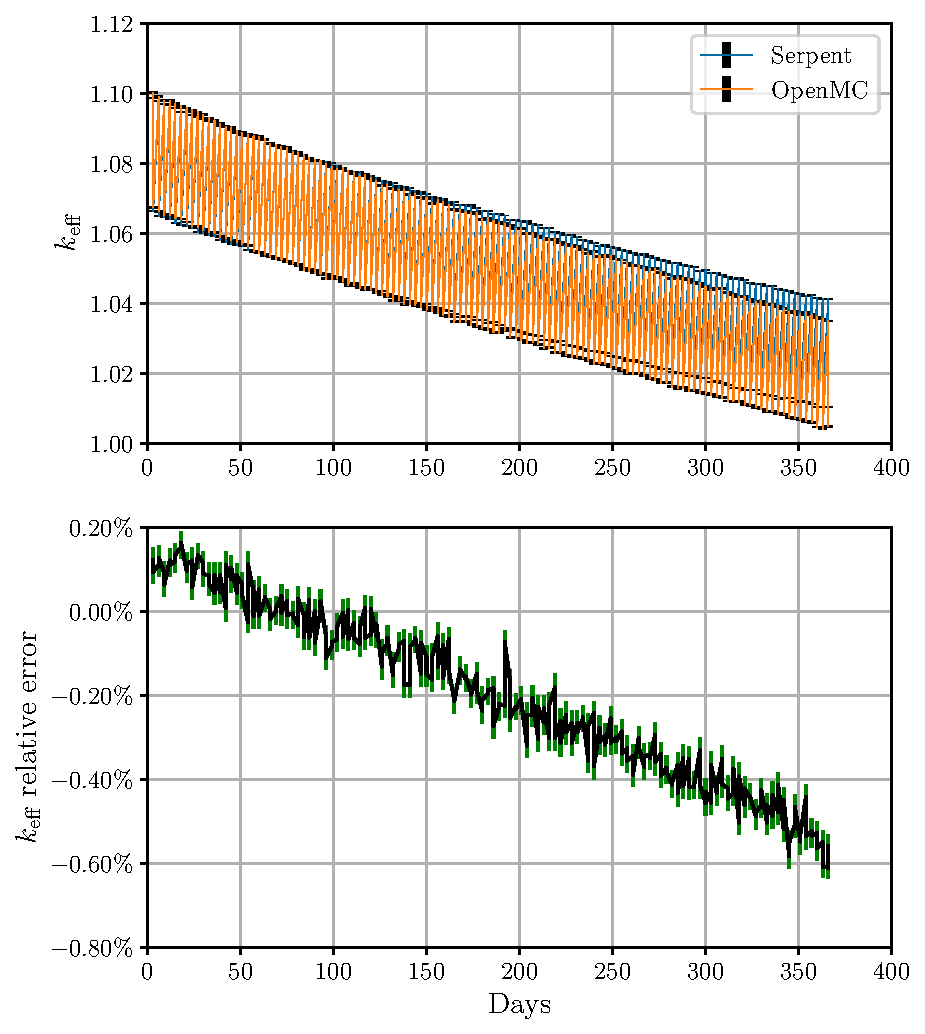
\includegraphics[width=0.8\linewidth]{figs/ch5/keff.pdf}
        \label{fig:keff}

    }\\
    \subfloat[][]{
        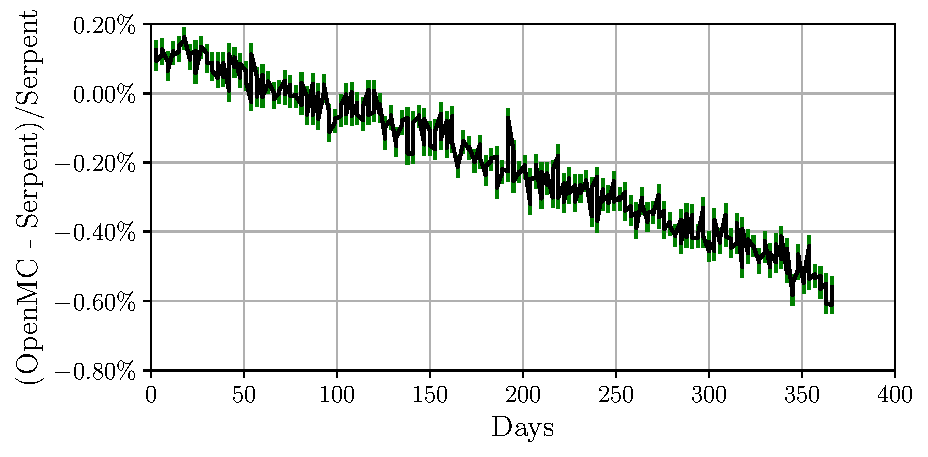
\includegraphics[width=0.8\linewidth]{figs/ch5/keff_error.pdf}
        \label{fig:keff_err}
    }
    \caption[$k_\text{eff}$ difference between \OpenMC and \SerpentTWO over time]{
        \subref{fig:keff} $k_\text{eff}$ difference between \OpenMC and \SerpentTWO over time;
        \subref{fig:keff_err} $k_\text{eff}$ relative difference between \OpenMC and \SerpentTWO 
        over time.
    }
    \label{fig:keff_sum}
\end{figure}

Figure \ref{fig:keff_sum} shows the change in $k_\text{eff}$ over time in the \OpenMC and \SerpentTWO
coupled simulations, as well as the relative difference between.
In Figure \ref{fig:keff}. the error bars are black, and in Figure
\ref{fig:keff_err}, they are green. For the first 15 days, the
$k_\text{eff}$ calculated by \OpenMC is slightly  higher than the 
$k_\text{eff}$ calculated by \SerpentTWO, with an average difference of around 35 pcm.
This is a very small difference, which makes sense as the material compositions should still
be more or less identical.

After 15 days, the $k_\text{eff}$ calculated by \OpenMC is becomes smaller than
the $k_\text{eff}$ calculated by \SerpentTWO. As time goes on, the difference
between the two grows at a rate of roughly 2 pcm per day. At the end of the simulation, the absolute
value of the relative difference is around 0.7\%, or 700 pcm. Notice the
oscillating behavior of $k_\text{eff}$. This is due to fuel reprocessing every 3 days.

% If we did not reprocess the fuel, the simulation
%would look like \ldots

\subsection{Nuclide compositions}
\label{sub:nuclide-compositions}

\begin{figure}[htpb]
    \centering
    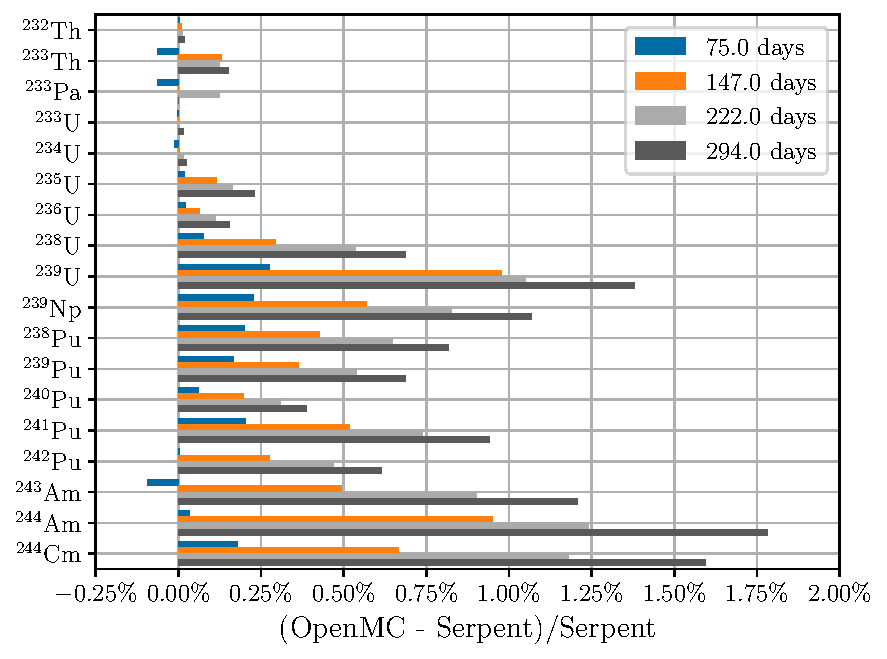
\includegraphics[width=0.8\textwidth]{figs/ch5/actinides.pdf}
    \caption[Relative difference of actinides mass in fuel at selected time steps]{Relative difference of actinides mass between \OpenMC and \SerpentTWO
    coupled simulations at 75, 147, 222, and 294 days. \ce{^{241}Am}, \ce^{{242}Am},
    \ce{^{242m}Am}, \ce{^{242}Cm},
    \ce{^{245}Cm}, and \ce{^{246}Cm} have been omitted here due to their high difference.
    See Section \ref{sub:actinide-analysis} for a discussion on these differences.}
    \label{fig:actinides}
\end{figure}

Figure \ref{fig:actinides} shows the relative error of actinide mass in the fuel
salt at several points in the simulation. \ce{^{241}Am}, \ce{^{242}Am},
\ce{^{242m}Am}, \ce{^{242}Cm}, \ce{^{245}Cm}, and \ce{^{246}Cm} have been omitted
from this figure due to their high differences at certain timesteps. We will analyse these
actinides in Section \ref{sub:actinide-analysis}. As time goes on, the error for
all actinides increases in magnitude. This is the most likely explanation for the constantly
increasing difference seen in $k_\text{eff}$. The difference for the actinides in
Figure \ref{fig:actinides} is around 2\% at the end of the simulation.

\begin{figure}[htpb]
    \centering
    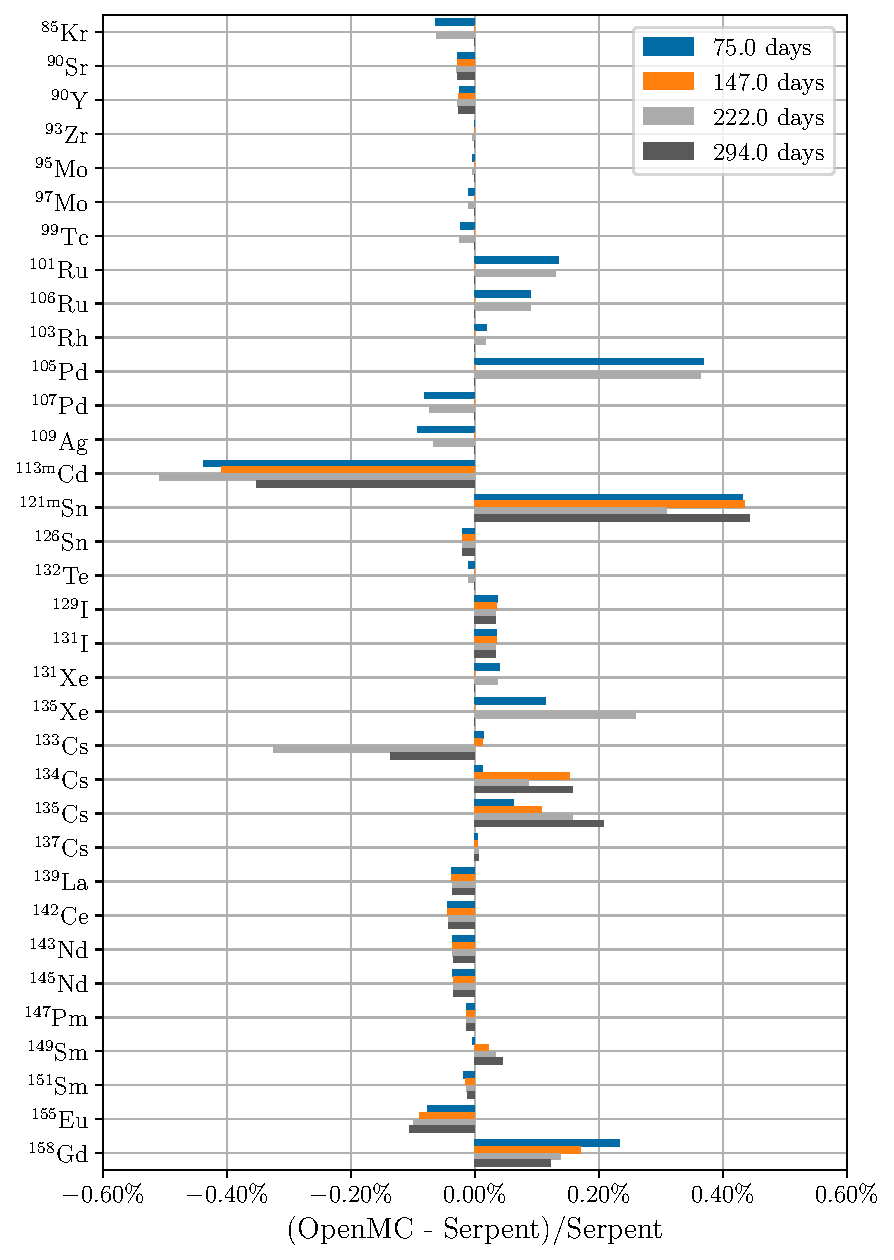
\includegraphics[width=0.8\textwidth]{figs/ch5/fission_products.pdf}
    \caption{Relative error of fission products mass in fuel}
    \label{fig:fission-products}
\end{figure}

Figure \ref{fig:fission-products} shows the relative error of fission product
mass in the fuel. The behavior of the error varies depending on the nuclide.
Overall, the difference between the \OpenMC and \SerpentTWO results are
very low, with no fission product having an error greater than 0.6\%, 
which makes sense as the fissionable actinide error is also very low. These
magnitudes are comparable with Romano et al (2021) \cite{romano_depletion_2021}, 
as seen in Figure \ref{fig:serpent-openmc-fp-interp}.\footnote{Romano
et al used MWd\/kg as their units, so it's not an apples to apples comparison.}

%go into detail about each nuclide?

\subsection{Actinide analysis}
\label{sub:actinide-analysis}

Our starting material only has \ce{^{233}U} for fissile material and \ce{^{232}Th} for fertile
material, and these two nuclides compose the majority of fissile and fertile material in the fuel,
respectively. Any difference in actinide nuclide composition between the two codes
most likely stems from a difference in \ce{^{233}U} or \ce{^{232}Th}, which are added
to the fuel after reprocessing.

\begin{figure}[htpb]
    \centering
    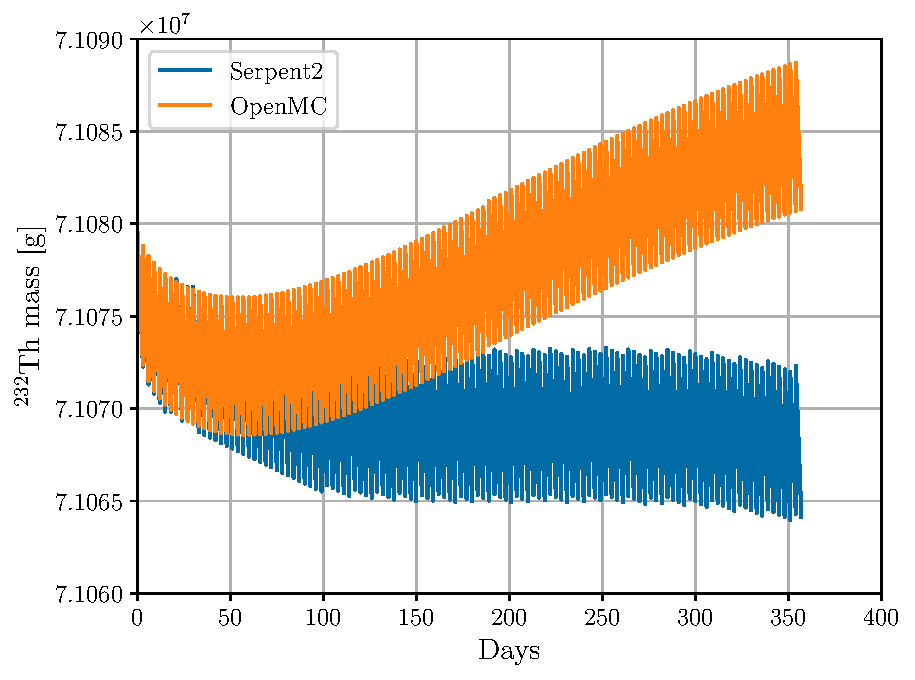
\includegraphics[width=0.8\textwidth]{figs/ch5/th232_mass.pdf}
    \caption{\ce{^{232}Th} mass over time for \OpenMC and \SerpentTWO}
    \label{fig:th232-mass}
\end{figure}

\begin{figure}[htpb]
    \centering
    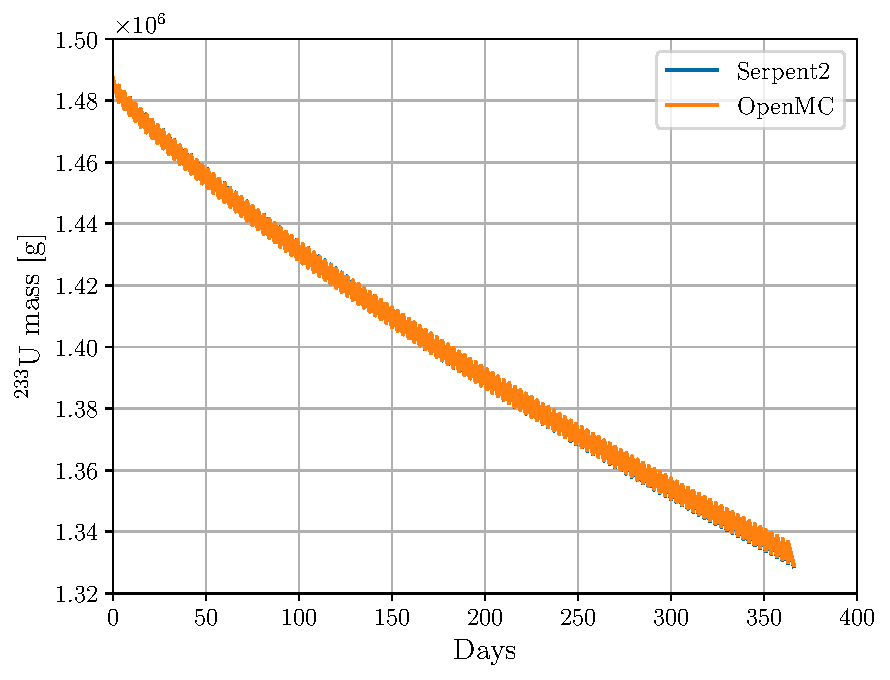
\includegraphics[width=0.8\textwidth]{figs/ch5/u233_mass.pdf}
    \caption{\ce{^{233}U} mass over time for \OpenMC and \SerpentTWO}
    \label{fig:u233-mass}
\end{figure}

Figure \ref{fig:th232-mass} and \ref{fig:u233-mass} show the mass of  \ce{^{232}Th} and
\ce{^{233}U} in the fuel, respectively. Whereas the \ce{^{233}U} mass is very similar
between \OpenMC and \SerpentTWO, there is a very large discrepancy in the \ce{^{232}Th}
mass. I find it unlikely that this is due to the reprocessing performed by \SaltProc.
Figure \ref{fig:th232-feed-mass} and \ref{fig:th232-feed-mass-diff} show the 
amount of \ce{^{232}Th} added to the fuel after each depletion step, and the
difference in that value between the \OpenMC and \SerpentTWO coupled simulations,
respectively. Notice that the total amount of \ce{^{232}Th} added to the fuel
is roughly the same in both the \OpenMC and \SerpentTWO, but the magnitude
of the difference shown in Figure \ref{fig:th232-mass} outpaces the amount of fuel
added shown in Figure \ref{fig:th232-feed-mass}. This indicates that there is another
mechanism at play causing this difference. Investigating this cause fully is outside the
scope of this thesis, however I suspect it is related to the small differences between the two
codes that I covered in Section \ref{sec:serpent-openmc-diff}.
I also suspect that there may be a slight difference in how \SerpentTWO is calculating it's
Q-values relative to how I calculated them for \OpenMC. I do want to bring attention to the fact
that the relative difference between the \OpenMC and \SerpentTWO \ce{^{232}Th} masses is very small,
less than 0.03\%, so this may just be a consequence of having so much \ce{^{232}Th} in the system.

% Maybe investigate the reaction rate?

\begin{figure}[htpb]
    \centering
    \subfloat[][]{
        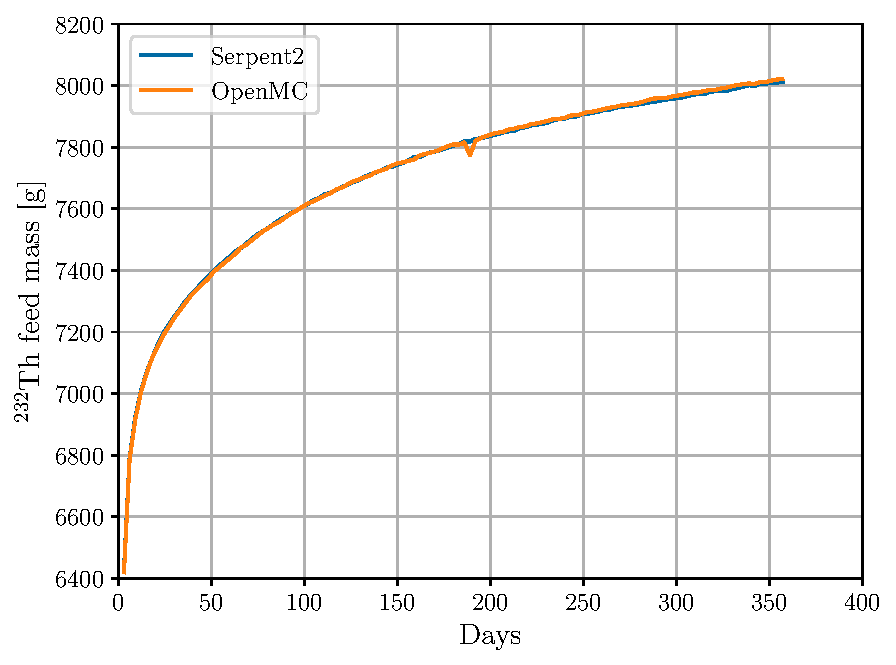
\includegraphics[width=0.5\linewidth]{figs/ch5/th232_feed_mass.pdf}
        \label{fig:th232-feed-mass}
    }
    \subfloat[][]{
        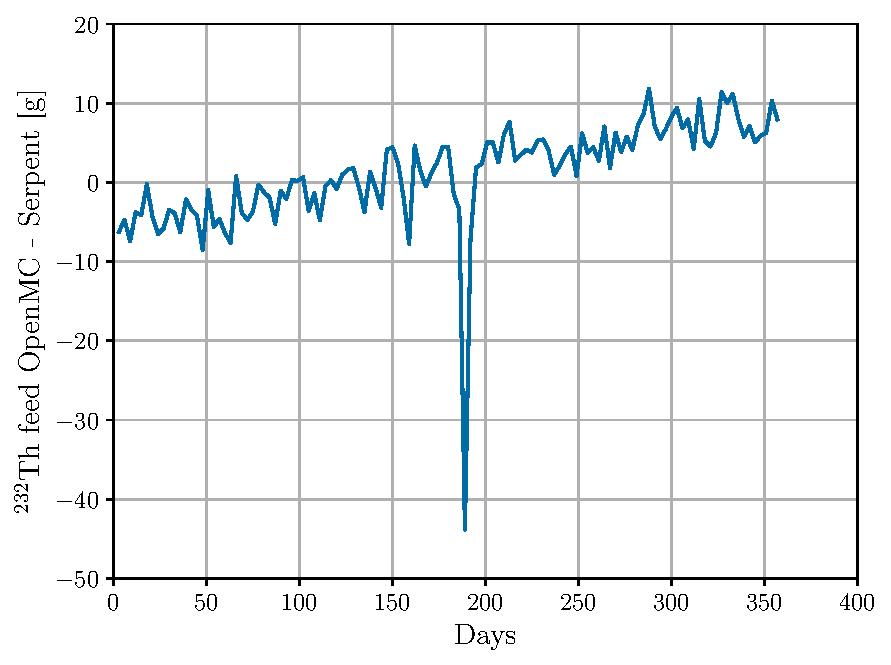
\includegraphics[width=0.5\linewidth]{figs/ch5/th232_feed_mass_diff.pdf}
        \label{fig:th232-feed-mass-diff}
    }
    \caption[\ce{^{232}Th} feed mass]{
    \subref{fig:th232-feed-mass} \ce{^{232}Th} feed mass;
    \subref{fig:th232-feed-mass-diff} \ce{^{232}Th} mass difference between \OpenMC and \SerpentTWO}
    \label{fig:cm242-mass}
\end{figure}

The difference in masses for \ce{^{241}Am}, \ce{^{242}Am}, \ce{^{242}Cm}, and \ce{^{243}Cm} are subject
to some strange numerical errors that result in very high differences at earlier depletion steps,
as seen in Figure \ref{fig:am-cm-mass-bol}. The differences converge to magnitudes similar to the
actinides in Figure \ref{fig:actinides}, as seen in Figure \ref{fig:am-cm-mass-diff}. As explained
in Section \ref{sec:saltproc-detail}, I added an experimental feature to \OpenMC to allow decay-only nuclides
to be added to a material for a depletion simulation. This feature has yet to be rigorously tested, so I am sure
there are some unintended side effects creating the differences between the \OpenMC and \SerpentTWO
simulations.

\begin{figure}[htpb]
    \centering
    \subfloat[][]{
        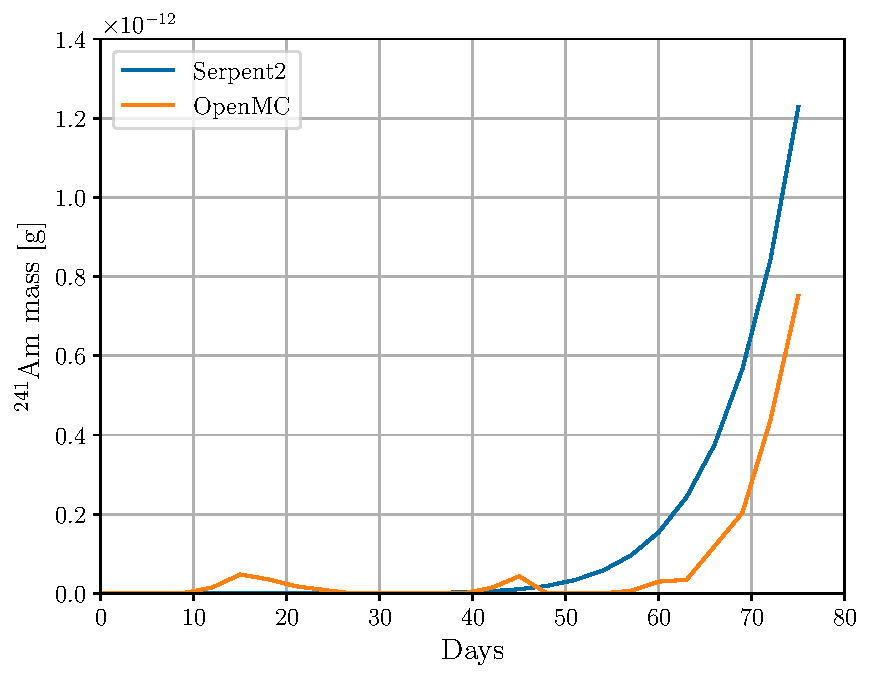
\includegraphics[width=0.5\linewidth]{figs/ch5/am241_mass_bol.pdf}
        \label{fig:am241-mass-bol}
    }
    \subfloat[][]{
        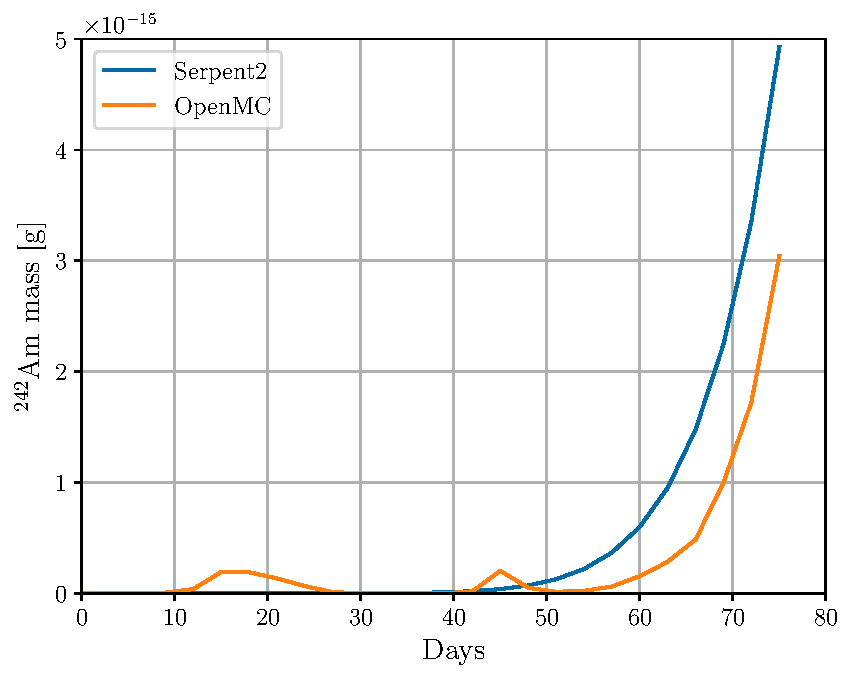
\includegraphics[width=0.5\linewidth]{figs/ch5/am242_mass_bol.pdf}
        \label{fig:am242-mass-bol}
    }
    \\
    \subfloat[][]{
        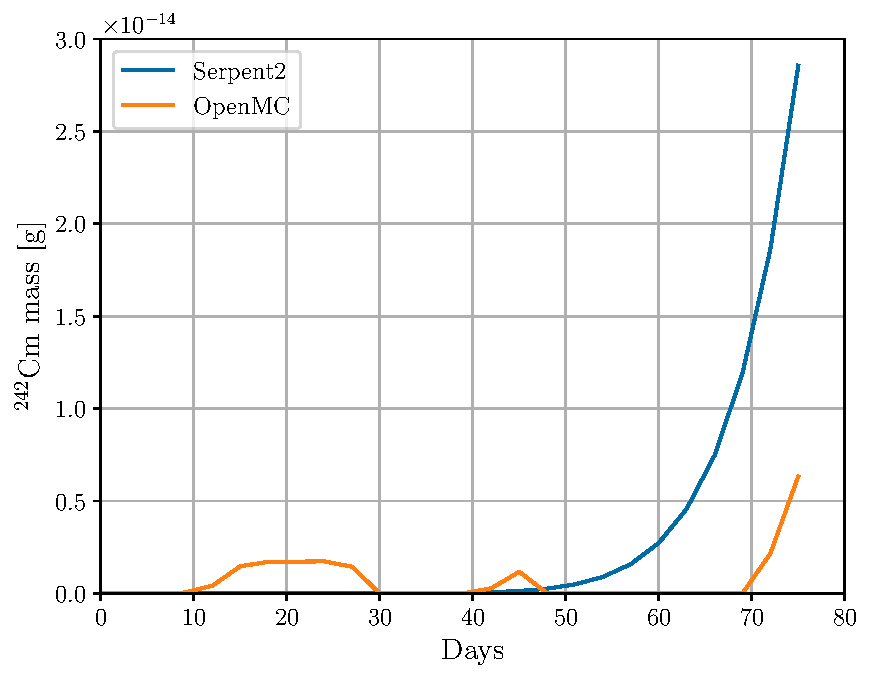
\includegraphics[width=0.5\linewidth]{figs/ch5/cm242_mass_bol.pdf}
        \label{fig:cm242-mass-bol}
    }
    \subfloat[][]{
        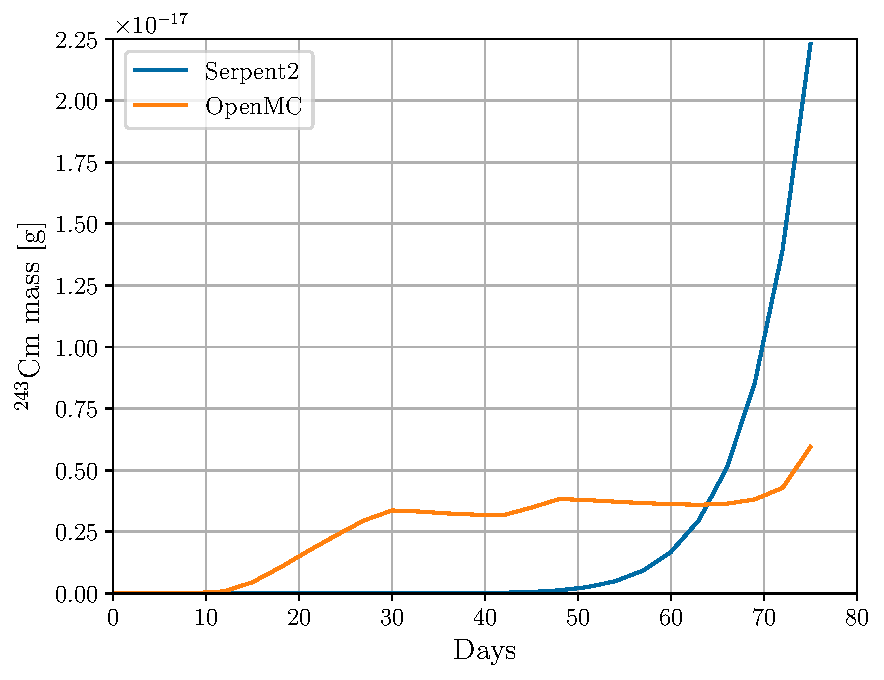
\includegraphics[width=0.5\linewidth]{figs/ch5/cm243_mass_bol.pdf}
        \label{fig:cm243-mass-bol}
    }
 
    \caption[\ce{^{241}Am}, \ce{^{242}Am}, \ce{^{242}Cm}, and \ce{^{243}Cm} mass up to 75 days]{
    \subref{fig:am241-mass-bol} \ce{^{241}Am} mass up to 75 days;
    \subref{fig:am242-mass-bol} \ce{^{242}Am} mass up to 75 days;
    \subref{fig:cm242-mass-bol} \ce{^{242}Cm} mass up to 75 days;
    \subref{fig:cm243-mass-bol} \ce{^{243}Cm} mass up to 75 days}
    \label{fig:am-cm-mass-bol}
\end{figure}


\begin{figure}[htpb]
    \centering
    \subfloat[][]{
        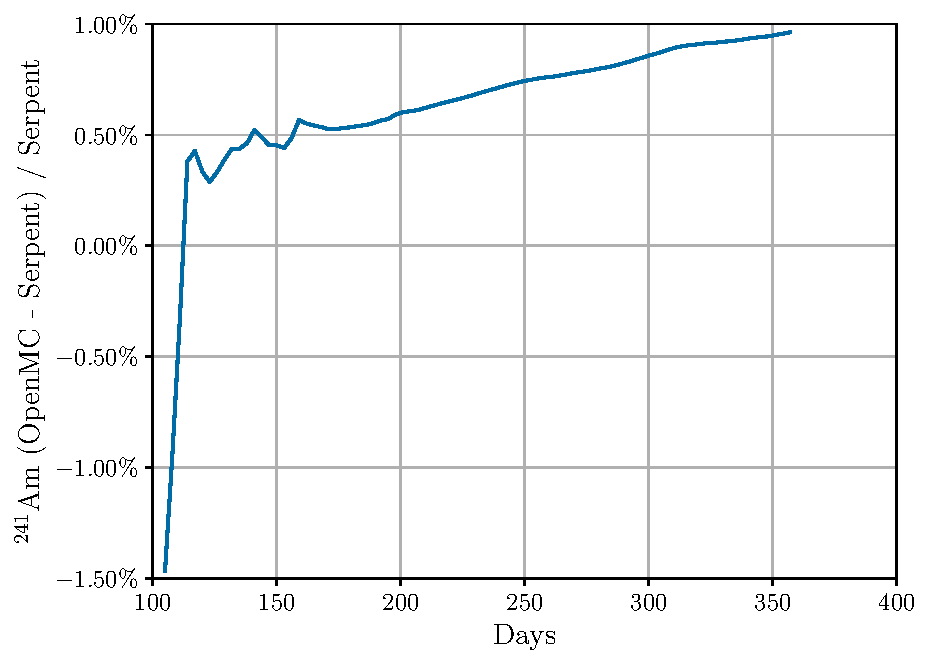
\includegraphics[width=0.5\linewidth]{figs/ch5/am241_mass_eol_diff.pdf}
        \label{fig:am241-mass-diff}
    }
    \subfloat[][]{
        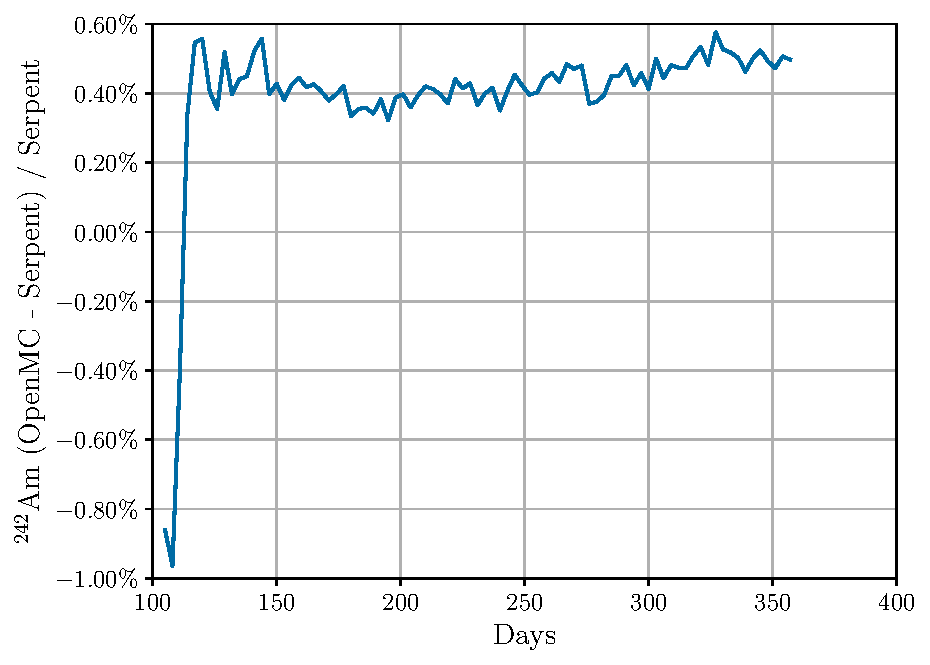
\includegraphics[width=0.5\linewidth]{figs/ch5/am242_mass_eol_diff.pdf}
        \label{fig:am242-mass-diff}
    }
    \\
    \subfloat[][]{
        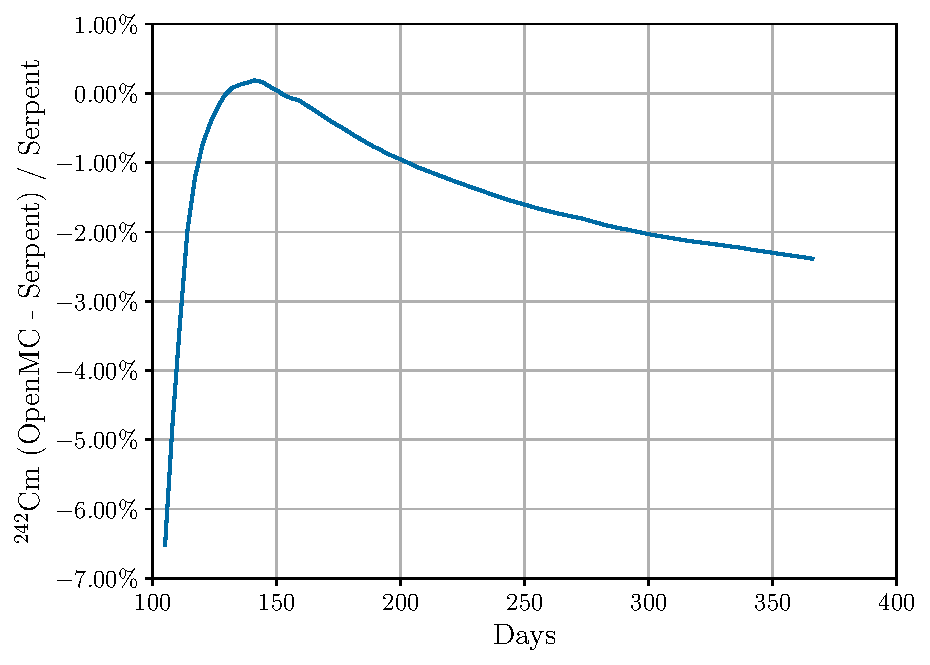
\includegraphics[width=0.5\linewidth]{figs/ch5/cm242_mass_eol_diff.pdf}
        \label{fig:cm242-mass-diff}
    }
    \subfloat[][]{
        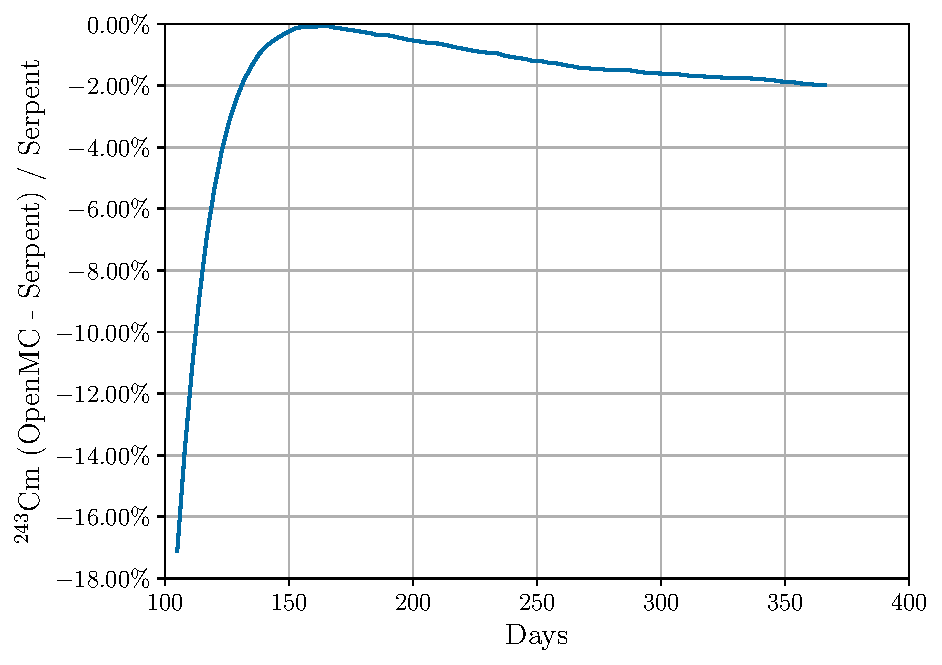
\includegraphics[width=0.5\linewidth]{figs/ch5/cm243_mass_eol_diff.pdf}
        \label{fig:cm243-mass-diff}
    }
 
    \caption[\ce{^{241}Am}, \ce{^{242}Am}, \ce{^{242}Cm}, and \ce{^{243}Cm} mass difference after 100 days]{
    \subref{fig:am241-mass-diff} \ce{^{241}Am} mass difference after 100 days;
    \subref{fig:am242-mass-diff} \ce{^{242}Am} mass difference after 100 days;
    \subref{fig:cm242-mass-diff} \ce{^{242}Cm} mass difference after 100 days;
    \subref{fig:cm243-mass-diff} \ce{^{243}Cm} mass difference after 100 days}
    \label{fig:am-cm-mass-diff}
\end{figure}

The differences in mass for \ce{^{242m}Am}, \ce{^{245}Cm}, and \ce{^{246}Cm} have the same kind of numerical errors, however
their differences do not converge as seen in Figure \ref{fig:am-cm-mass-eol}.
For \ce{^{245}Cm} and \ce{^{246}Cm}, I hypothesize they just need more time to build up to
concentrations where they would converge. However, there appears to be an actual difference
in the way \OpenMC and \SerpentTWO are producing and consuming \ce{^{242m}Am}. As with
\ce{^{232}Th}, this may be due to a slight difference in fission-Q values.

\begin{figure}[htpb]
    \centering
    \subfloat[][]{
        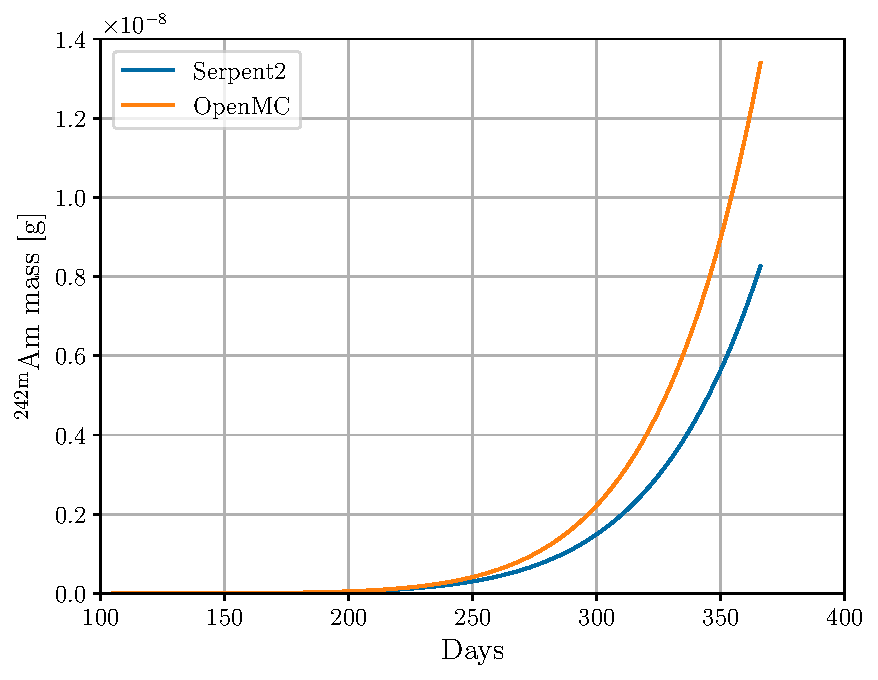
\includegraphics[width=0.5\linewidth]{figs/ch5/am242m_mass_eol.pdf}
        \label{fig:am242m-mass-eol}
    }
    \subfloat[][]{
        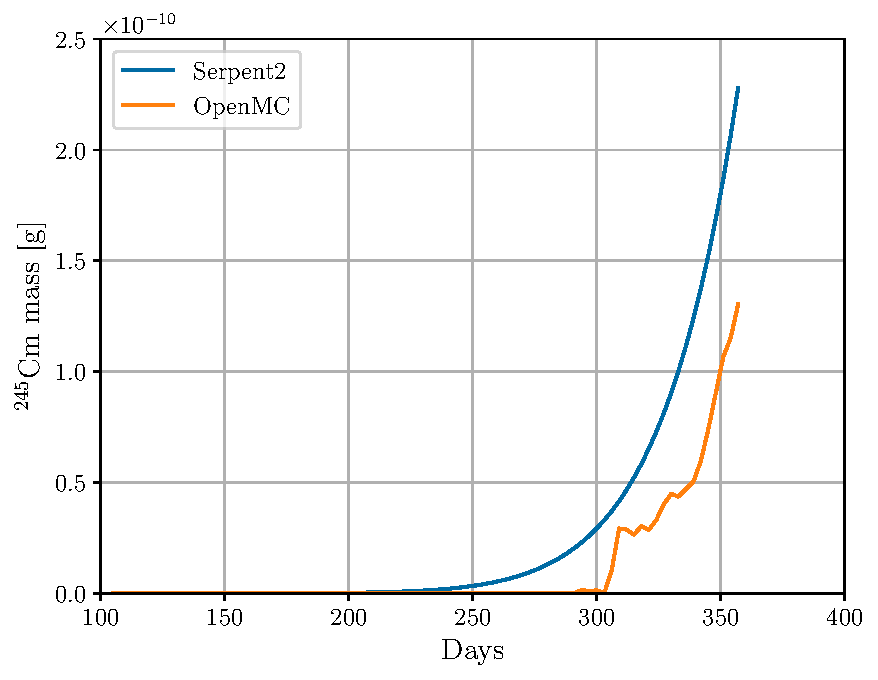
\includegraphics[width=0.5\linewidth]{figs/ch5/cm245_mass_eol.pdf}
        \label{fig:cm245-mass-eol}
    }
    \\
    \subfloat[][]{
        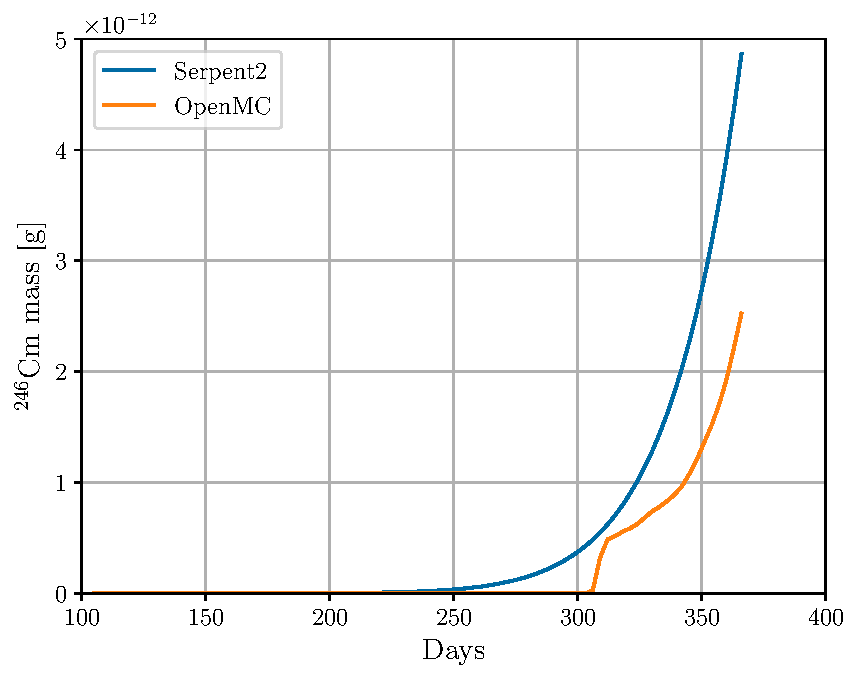
\includegraphics[width=0.5\linewidth]{figs/ch5/cm246_mass_eol.pdf}
        \label{fig:cm246-mass-eol}
    }
    \caption[\ce{^{241m}Am}, \ce{^{245}Cm}, and \ce{^{246}Cm} mass after to 100 days]{
    \subref{fig:am242m-mass-eol} \ce{^{242m}Am} mass after 100 days;
    \subref{fig:cm245-mass-eol} \ce{^{245}Cm} mass after 100 days;
    \subref{fig:cm246-mass-eol} \ce{^{246}Cm} mass after 100 days}
    \label{fig:am-cm-mass-eol}
\end{figure}


